\graphicspath{{../images/algorithm/}}
\chapter{Экспериментальные результаты}
\section{Поиск и обработка исходных данных для оценки работы алгоритма}
\cite{asedb2001}

\cite{kortemme_alascan_datasets}
\cite{sdr1}
%\todo{глава не готова}
\section{Пример работы итеративного алгоритма выбора протяженных регионов}
Для оценки корректности работы алгоритма на каждом из этапов проводился визуальный контроль выбираемых аминокислот с использованием средств визуализации приложения PyMol ~\cite{pymol}.

Далее приведены несколько скриншотов с L и H цепями антитела (структура с идентификатором 2OSL, с исключенными молекулами воды) с разных ракурсов, на которых выделены разными цветами аминокислоты, добавляемые к региону для аланинового сканирования на разных этапах:
\begin{itemize}

\item желтым цветом изображена L-цепь, на ней голубым цветом выделены аминокислоты, содержащие атомы, которые попали в начальное отобранное множество треугольников выпуклой оболочки;

\item синим цветом выделены аминокислоты, атомы которых попали в выделенную область на этапе поиска карманов;

\item красным цветом выделены участки цепочки, которые были добавлены в результате добавления петель, частично попавших в выделенный регион на одном из предыдущих этапов.
\end{itemize}

\begin{figure}
%\resizebox{0.8\textwidth}{!}{
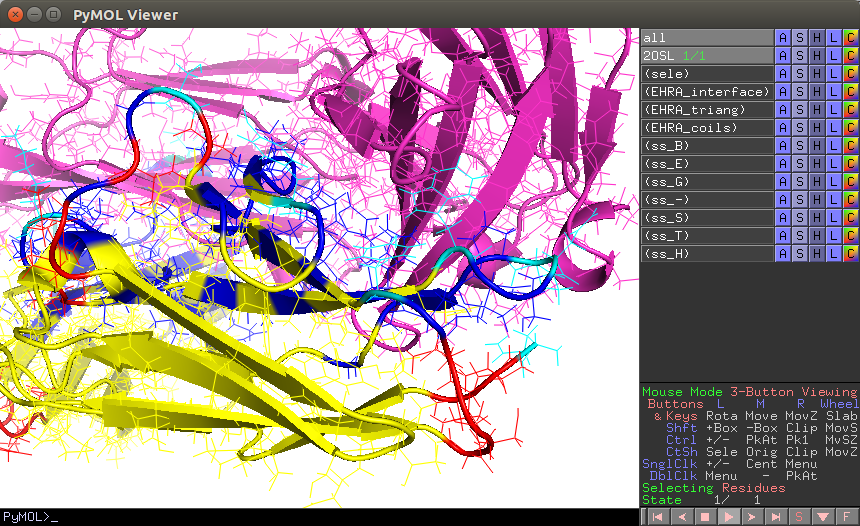
\includegraphics[width=\linewidth]{loops1.png}
%}

\caption{\small{[Computation of tunnels in protein molecules using
Delaunay triangulation, P.Medek, et al., 2007]
 }}
\label{fig:loops1}
\end{figure}


\begin{figure}
%\resizebox{0.8\textwidth}{!}{
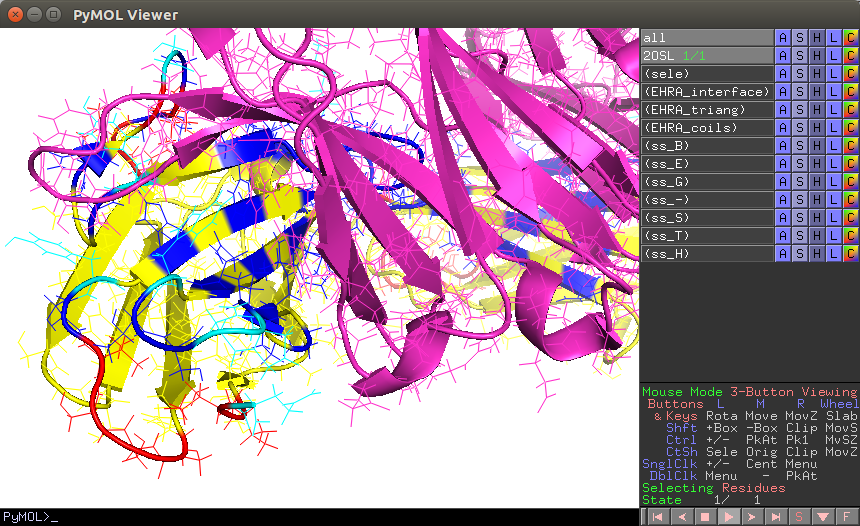
\includegraphics[width=\linewidth]{loops2.png}
%}

\caption{\small{[Computation of tunnels in protein molecules using
Delaunay triangulation, P.Medek, et al., 2007]
 }}
\label{fig:loops2}
\end{figure}



На последнем из приведенных скриншотов в нижней части изображения видна петля, которая удалена от интерфейса взаимодействия, но при этом один из атомов ее аминокислот по удачному стечению обстоятельств попал в множество отобранных треугольников выпуклой оболочки, за счет чего петля попала целиком.

%\todo{И это наводит на мысль о том, что изначальный выбор аминокислот не так хорош. Возможно, стоит использовать граф Габриэля? }


\begin{figure}
%\resizebox{0.8\textwidth}{!}{
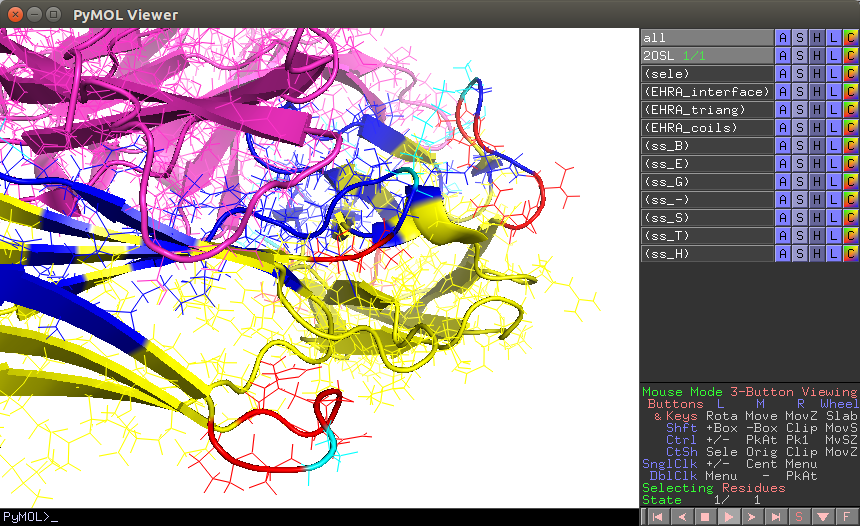
\includegraphics[width=\linewidth]{loops3.png}
%}

\caption{\small{[Computation of tunnels in protein molecules using
Delaunay triangulation, P.Medek, et al., 2007]
 }}
\label{fig:loops3}
\end{figure}



%Посередине петля полностью желтая - но это из-за способа, которым добавлялись карманы.


\begin{figure}
%\resizebox{0.8\textwidth}{!}{
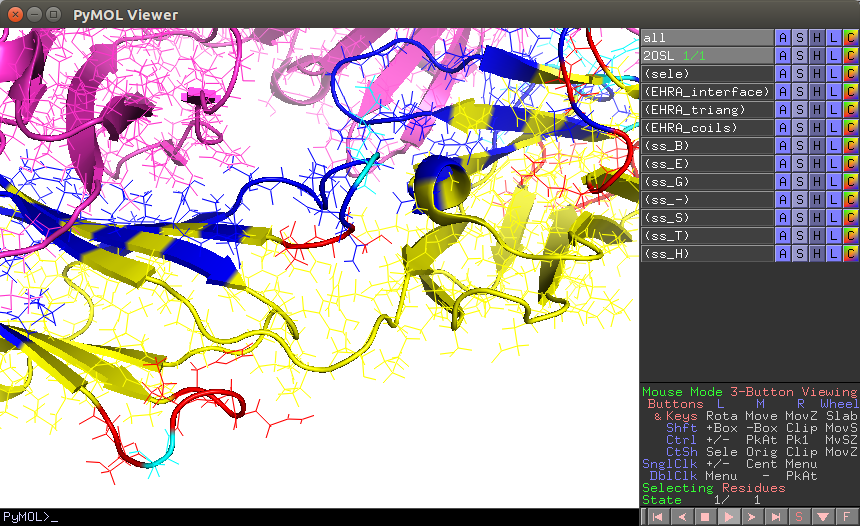
\includegraphics[width=\linewidth]{loops4.png}
%}

\caption{\small{[Computation of tunnels in protein molecules using
Delaunay triangulation, P.Medek, et al., 2007]
 }}
\label{fig:loops4}
\end{figure}


\newpage
%\section{Протокол аланинового сканирования}
% http://www.bakerlab.org/system/files/kortemme04B.pdf
% - картинка отсюда с страницы 3
%\todo{-нужна картинка про rosetta alascan protocol }

%В работе \cite{kortemme2002} показано, что (сказать про функцию энергии для компьютерного моделирования аланинового сканирования)

%\todo{-описание того, в какой части предполагается использовать модиф регионы}
%\vspace{10cm}


\newpage
\section{Пример работы на структурах с известными результатами  экспериментального аланинового сканирования}
%Уже обработанные данные есть здесь: \cite{kortemme_alascan_datasets}

%Картинка \cite{benchmark_img} но я не уверена, можно ли ее приводить без разрешения

%\todo{- картинка с схемой работы скрипта}

%\todo{- красивая табличка, с процентом аминокислот в цепочке, попавших в регион, а также попавшими и не попавшими хотспотами.}
%Описание таблички (нужно для корректного вывода в скрипте)
% 1. идентификатор файла pdb
% 2. мутируемая цепь
% 3. цепь\ лиганд, взаимодействие с которым оценивается
% 4. длина цепочки, длина региона, число замаскированных амк
% 5.
%\\

%\todo{-написать скрипт, который для данного pdb и пары цепочек проводит ala-scan по всем позициям и сравнивает методы, которые используются для фильтрации аминокислот.}

%\todo{сделать табличку по данным asedb и bid, и для того, что нет (хотспоты искать с помощью протокола аланинового сканирования, в табличке рисовать циферки). если есть амк, которые не нашлись,}
%\vspace{10cm}
Был проведен поиск регионов для структур, содержащихся в наборе данных для бенчмаркинга Kortemme \& Baker \cite{kortemme_alascan_datasets} (без учета воды, изначальный набор атомов выпуклой оболочки определялся со значением отсечки по расстоянию 5 \AA{}). Результаты работы скрипта для двухцепочечных структур приведены в таблице:
\begin{table}[h]
\begin{center}
	\caption{Сравнение вычисленных синтенных блоков}
	\label{tab:comparison}
\begin{tabular}{|c|c|c|c|c|c|c|c|c|c|}
\hline
 PDB & chain & P+N & TP+FP & TP & TP+FN & FN & TPR & ACC & MCC\\
 \hline
  1 & 2 & 3 & 4 & 5 & 6 & 7 & 8 & 9 & 10\\
 \hline
1A22 & A & 180 & 114 & 29 & 29 & 0 & 1.00 & 0.5874 & 0.3636\\
1A22 & B & 192 & 177 & 36 & 36 & 0 & 1.00 &
0.4000 & 0.2435
\\
1BXI & A & 83 & 70& 29& 30& 1 & 0.97 &
0.6585 & 0.4560
\\
1DFJ & I & 456 & 255& 11& 14& 3 & 0.79 &
0.4969 & 0.0913
\\
1F47 & A & 17 & 17&	9& 9& 0 & 1.00 &
0.7576 & 0.5941
\\
1FC2 & C & 45 & 44&	3& 3& 0 & 1.00 &
0.0889 & 0.0403
\\
2PTC & I & 58 & 55&	1& 1& 0 & 1.00 &
0.4194 & 0.0867\\
\hline
\end{tabular}
\end{center}
\end{table}
\\[10pt]
Расшифровка: 
\begin{itemize}
\item графы 1 и 2 - имя файла со структурой в Protein Data Bank и цепочки, на которой расположены энергетически значимые аминокислоты;
\item 3 графа - число аминокислот в цепочке;
\item 4 графа = число аминокислот, выбранных алгоритмом поиска регионов;
\item 5 графа - число аминокислот-хотспотов на цепочке по данным из базы данных;
\item 6 графа - число аминокислот-хотспотов, находящихся в выбранном алгоритмом регионе;
\item 7 графа - число аминокислот-хотспотов, которые есть в базе, но которые не попали в выбранный протяженный регион;
\item следующие графы - рассчитанные характеристики.
\end{itemize}

На следующем скриншоте приведена цепочка A структуры 1BXI, с выделенными на ней областями. Красным цветом показаны элементы вторичной структуры, попавшие в выделенный регион, желтым цветом изображена аминокислота, которая является энергетически значимой, но которая в выделенный регион не попала.

\begin{figure}

%\resizebox{0.8\textwidth}{!}{
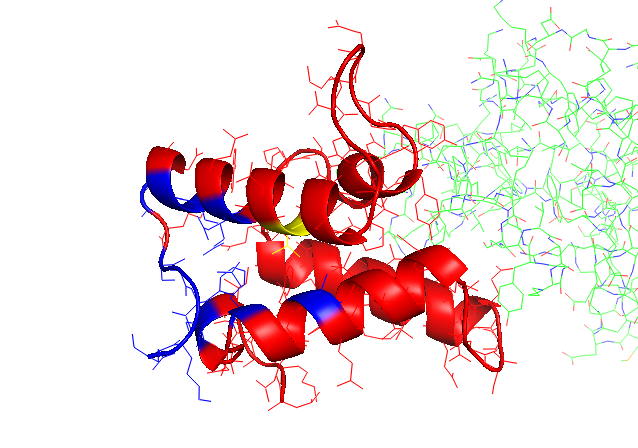
\includegraphics[width=\linewidth]{1BXI.png}
%}
\caption{\small{[Computation of tunnels in protein molecules using
Delaunay triangulation, P.Medek, et al., 2007]
 }}
\label{fig:1BXI}

\end{figure}

В случае второй структуры, у которой в выделенный протяженный регион попали не все энергетически значимые аминокислоты (1DFJ), скриншот выглядит так (энергетически значимые аминокислоты, не попавшие в регион - красные, выделенный регион - желтым цветом, остальная часть цепочки показана голубым цветом):


\begin{figure}[h]
%\resizebox{0.8\textwidth}{!}{
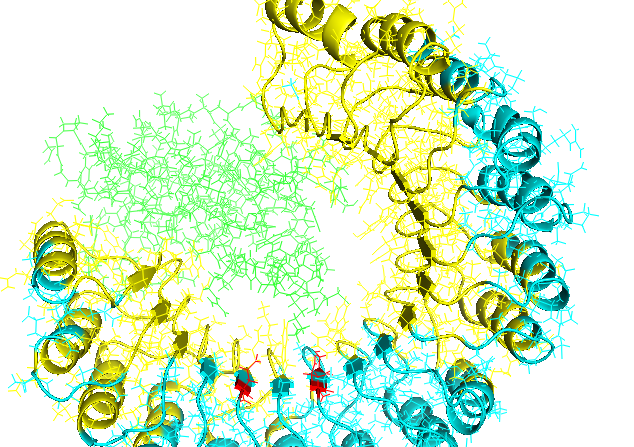
\includegraphics[width=\linewidth]{1DFJ.png}
%}

\caption{\small{Структура с идентификатором  1DFJ в Protein Data Bank
 }}
\label{fig:1DFJ}
\end{figure}



Такой результат объясняется тем, что интерфейс взаимодействия расположен в кармане, а также текущим способом поиска карманов, используемым в алгоритме.

В остальных случаях для двух цепочек энергетически горячие аминокислоты нашлись все (TPR=1). Маленькие значения точности (ACC) и коэффициента корреляции Мэтьюса можно объяснить тем, что для начального выбора атомных центров-вершин выпуклой оболочки берется фиксированная отсечка по расстоянию, что может приводить в отдельных случаях к выбору в состав региона для сканирования большей части цепочки или всей цепочки.

С файлами, которые содержали более 2 цепочек, была проведена аналогичная процедура с усложнением: энергетически значимые аминокислоты сгруппированы по цепочкам, для каждой из этих цепочек парная цепочка, относительно которой выбирался регион, была определена как одна из оставшихся цепочек. Корректные результаты работы приведены в таблице (расшифровка граф аналогична расшифровке в предыдущем случае):
\begin{table}
\begin{center}
	\caption{Сравнение вычисленных синтенных блоков}
\resizebox{\linewidth}{!}{
\begin{tabular}{|c|c|c|c|c|c|c|c|c|c|c|}
\hline
pdb & chain1 & chain2 & P+N & TP+FP & TP+FN & TP & TPR & ACC & MCC \\
\hline
1CBW & D & C & 79 & 57 & 8 & 8 & 1.00 & 0.3797 & 0.2085\\
1CBW & D & B & 79 & 58 & 8 & 8 & 1.00 & 0.3671& 0.2020\\
1CBW & D & G & 79 & 52 & 8 & 8 & 1.00 & 0.4430 & 0.2419 \\
1CBW & D & H & 79 & 43 & 8 & 5 & 0.63 & 0.4810 & 0.0544 \\
1CBW & D & I & 79 & 54 & 8 & 8 & 1.00 & 0.4177 & 0.2284\\
\hline
1DAN & U & L & 162 & 113 & 23 & 23 & 1.00 & 0.4444 & 0.2679\\
1DAN & U & H & 162 & 93 & 23 & 18 & 0.78 & 0.5062 & 0.1715\\
1DAN & U & T & 162 & 108 & 23 & 21 & 0.91 & 0.4506 & 0.2126\\
1DAN & T & L & 115 & 75 & 20 & 20 & 1.00 & 0.5217 & 0.3351\\
1DAN & T & H & 115 & 68 & 20 & 14 & 0.70 & 0.4783 & 0.1015\\
1DAN & T & U & 115 & 75 & 20 & 20 & 1.00 & 0.5217 & 0.3351\\
\hline
1AHW & C & A & 200 & 176 & 8 & 8 & 1.00 & 0.1600 & 0.0754\\
1AHW & C & B & 200 & 190 & 8 & 8 & 1.00 & 0.0900 & 0.0468\\
\hline
1JCK & B & A & 239 & 200 & 9 & 9 & 1.00 & 0.2008 & 0.0874\\
1JCK & B & C & 239 & 137 & 9 & 8 & 0.89 & 0.4561 & 0.1262\\
\hline
1BRS & A & B & 253 & 81 & 8 & 7 & 0.88 & 0.7036 & 0.2149\\
1BRS & A & C & 253 & 72 & 8 & 3 & 0.38 & 0.7075 & 0.0362\\
1BRS & A & D & 253 & 92 & 8 & 8 & 1.00 & 0,6680 & 0.2390 \\
1BRS & D & A & 164 & 77 & 6 & 6 & 1.00 & 0.5671 & 0.2071\\
\hline
1DN2 & A & E & 248 & 178 & 3 & 3 & 1.00 & 0.2944 & 0.0694\\
1DN2 & A & B & 248 & 189 & 3 & 3 & 1.00 & 0.2500 & 0.0618\\
\hline
1A4Y & A & B & 516 & 282 & 14 & 14 & 1.00	& 0.4806 & 0.1521\\
1A4Y & A & D & 516 & 354 & 14 & 11 & 0.79 & 0.3295 & 0.0359\\
1A4Y & A & E & 516 & 302 & 14 & 9 & 0.64 & 0.4225 & 0.0195\\
1A4Y & B & A & 141 & 111 & 14 & 14 & 1.00 & 0.3121 & 0.1726\\
\hline
\end{tabular}
}
\end{center}
\end{table}
\\[10pt]

Видно, что TPR -высокий, это означает, что в большинстве случаев все энергетически важные аминокислоты попали в выбранный протяженный регион. Точность низкая потому, что в состав протяженного региона попали больше половины аминокислот цепочки.

На некоторых структурах, содержащих более 2 цепочек, были получены некорректные результаты. Таких структур получилось 4, с идентификаторами 1JRH, 1GC1, 1NMB и 3HFM. %Планирую добавить анализ этих результатов+сравнение с тупым выбором аминокислот по расстоянию
